% TO-DO:
% * Actions = all possible transtions in RL
% * In RL, Q-learning is still unclear -- currently I'm using NN = transition F(x)
%   -- U(x) -> U(x') so it seems that generalization can occur in Q-space (?)
% * Structure of the turnstile is an important feature of the transition F(x)
% * Explain difference with AIXI
% * "inward" vs "outward"

\documentclass[orivec]{llncs}
\usepackage{graphicx}
\usepackage{amsmath}		% for "cases"
\usepackage{amsfonts}		% for frakur fonts
\usepackage{mathrsfs}		% for curly "E" error symbol
\usepackage{float}
\usepackage[most]{tcolorbox}% for wrapping example in color box
\usepackage{wrapfig}		% wrap figure beside text, used in example
\usepackage{tikz-cd}		% commutative diagrams
% \usepackage{amsfonts}
\usepackage{enumitem}       % for using (A),(B),(C) in items...
\usepackage{amssymb}		% for \multimap, \updownarrow, \bigstar
\usepackage{turnstile}		% longer turnstiles
\usepackage{sectsty}		% change section color
\usepackage{hyperref}		% refs, links become clickable
\usepackage{url}			% for urls in bibliography
\usepackage[normalem]{ulem} % underline unbroken with \uline
\usepackage[numbers,sectionbib]{natbib}% if we use \package{url} we need to use natbib style

%\def\chinchin{yes}          % ********** 用中文 *********
% *************** Delete when not using Chinese or colors **********************
\ifdefined\chinchin
	\usepackage{xeCJK}
	\setCJKmainfont[BoldFont=SimHei,ItalicFont=KaiTi]{SimSun}
\fi
\usepackage{color}
%\newcommand{\emp}[1]{\textbf{\textcolor{blue}{#1}}}
\newcommand{\emp}[1]{\textbf{#1}}

\sectionfont{\color{blue}} 
\subsectionfont{\color{blue}} 
\subsubsectionfont{\color{blue}} 
\definecolor{green}{rgb}{0,0.7,0}
\definecolor{grey}{rgb}{0.95,0.95,0.95}

\usepackage{geometry}		% change paper size
\geometry{
  a4paper,         % or letterpaper
  textwidth=18cm,  % llncs has 12.2cm
  textheight=27cm, % llncs has 19.3cm
  heightrounded,   % integer number of lines
  hratio=1:1,      % horizontally centered
  vratio=2:3,      % not vertically centered
}
\usepackage[fontsize=13pt]{scrextend}

\newcommand{\tikzmark}[1]{\tikz[overlay,remember picture] \node (#1) {};}

\newcommand{\vect}[1]{\boldsymbol{#1}}
\newcommand*\sigmoid{\vcenter{\hbox{
\includegraphics{sigmoid.png}}}}
\newcommand*\rectifier{\vcenter{\hbox{\includegraphics{rectifier.png}}}}
\newcommand*\KB{\vcenter{\hbox{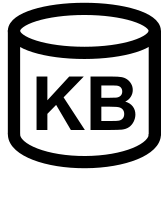
\includegraphics{KB-symbol.png}}}}
\newcommand*\KBsmall{\vcenter{\hbox{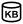
\includegraphics{KB-symbol2.png}}}}
\newcommand*\Eye{\vcenter{\hbox{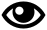
\includegraphics{../eye-symbol.png}}}}
\newcommand*\NN{\vcenter{\hbox{
\includegraphics{NN-symbol.png}}}}
\newcommand*\Graph{\vcenter{\hbox{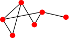
\includegraphics{algebraic-model.png}}}}
\newcommand{\dashh}{\textemdash~}
\newcommand{\english}[1]{\mbox{\textit{#1}}}
\newcommand{\tab}{\hspace*{2cm}}

% ***** Boxed variables inside math equations
% \newcommand*{\boxedcolor}{black}
\makeatletter
% \renewcommand{\boxed}[1]{\textcolor{\boxedcolor}{%
% \fbox{\normalcolor\m@th$\displaystyle#1$}}}
% \setlength{\fboxsep}{1pt}
\renewcommand{\boxed}[1]{\fbox{\m@th$\displaystyle\scalebox{0.9}{#1}$} \,}
\makeatother

\overfullrule=0mm

\newsavebox{\MyName}
\savebox{\MyName}{
\includegraphics[scale=0.6]{YKY.png}}

\title{White paper}
%\normalsize{-- a minimalist cognitive architecture combining\\
%reinforcement learning and deep learning}}
\titlerunning{White paper}
\author{\usebox{\MyName} (King-Yin Yan)
% \\ \footnotesize{General.Intelligence@Gmail.com}
%\and
%Ben Goertzel
%\and
%Juan Carlos Kuri Pinto
}
\institute{General.Intelligence@Gmail.com}
\date{\today}

\begin{document}
\let\labelitemi\labelitemii

\maketitle

\noindent
\makebox[\linewidth]{\small \today}

\setlength{\parindent}{0em}
\setlength{\parskip}{2.8ex plus0.8ex minus0.8ex}
% \setlength{\parskip}{2.8ex}

\begin{abstract}
	This paper describes a cognitive architecture for common-sense reasoning.
% 这篇是背景,介绍一个基於 \textbf{增强学习} 和 \textbf{深度学习} 的极简约的 cognitive architecture,它在数学上是一个Hamiltonian 系统,而其 Lagrangian 对应於智能系统的「奖励」或「欲望」的价值。 经典逻辑 AI 的技巧可以搬到这个 setting 之下,而连续时间化之后,可以用上微分几何的技巧。 传统的「逻辑 AI 知识表述」被新的表述法取代,后者的结构是由神经网络的深度学习「诱导」出来的。
%This is the first of a series of papers, introducing a minimalist cognitive architecture based on reinforcement learning and deep learning.  The system consists of an iterative function whose role is analogous to the consequence operator ($\vdash$) in logic.  It is fascinating to note this is a Hamiltonian system, whose Lagrangian corresponds to the value of ``desires'' or ``rewards'' for the intelligent agent;  but the usefulness of this idea is as yet unknown.  More importantly, the structure of classical logic-based AI can be transferred to the neural setting, the topic of our 2nd paper.
%Its continuous limit can be described by differential geometry.  The old-fashioned logic-based knowledge representation with discrete propositions is abandoned in favor of a representation induced by deep neural learning.
% The problem of general intelligence can be described and solved in the logic-based AI paradigm, but the main obstacle is that learning is too slow.  The logic-based knowledge representation with discrete propositions is abandoned in favor of a neural-based ``amorphous'' representation induced from the top down, using a deep neural network (DNN).  The DNN acts iteratively on a state space (the ``mental state''), forming a dynamical system.  This system is in turn controlled by reinforcement learning, ``navigating'' the space of mental states as in a maze.
\end{abstract}

%\begin{keywords}
%reinforcement learning, control theory, deep learning, cognitive architecture
%\end{keywords}

\setcounter{section}{-1}
\section{Introduction}
% \label{sec:0}

The architecture for \textbf{visual recognition} is:
\begin{equation}
\vcenter{\hbox{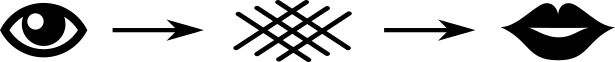
\includegraphics[scale=0.6]{vision-architecture.png}}}
\end{equation}
Our basic architecture is:
\begin{equation}
\vcenter{\hbox{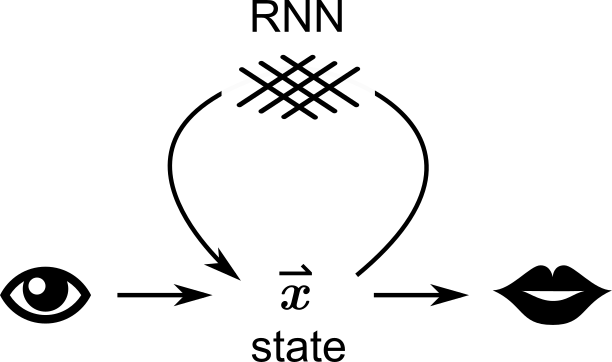
\includegraphics[scale=0.6]{basic-architecture.png}}}
\label{basic-arch}
\end{equation}

$\NN$ = [deep] neural network, trained via reinforcement learning

$\Graph$ = mental state / working memory

The main problems we need to solve:
\begin{enumerate}[label=(\Alph*)]
	\item How to enable a neural network to act on a graph structure (that does not easily fit into a fixed-length vector)?
	\item How to achieve an ability that I call ``learn by being told''? \\
	This is related to the functional closure $\mathbb{X} \simeq \mathbb{X}^{\mathbb{X}}$ which gives a Cartesian-closed category
	\item How to incorporate \textbf{episodic memory} into the basic architecture (\ref{basic-arch})? \\
	Episodic memory may be essential for the learning of common-sense (eg. the need to process \textbf{stories}).
\end{enumerate}

\ifdefined\chinchin
Deep learning 所带来的好处是: 它可以在 ``multifarious''(「纷纭繁杂」) 的资料中 factorize 出一些 intermediate features,从而将庞大的资料分类成数目较少的类别。 这种分类法是旧式 AI 里没有的,例如 decision trees 的分类法,资料在切割之后不再相关。 但神经网络像一些「拉面条」那样,在 hidden layers 中产生出 representation learning,这是以前的技术没有的。 
\else
The advantage brought by deep learning is that it is capable of factorizing \textbf{intermediate features} out of ``multifarious'' data, classifying them into a relatively smaller number of classes.  This capability is absent in traditional AI.  For example, in decision trees, once classes are split they are processed \textit{separately}.  Whereas neural networks have layers like continually ``stretching noodles'', they can do what is called \textbf{representation learning} in the hidden layers.  This technology was unavailable before.
\fi

The reason why I believe we can build AGI, is because we can use a deep network to emulate the following function:
\begin{equation}
\NN \quad \Longleftrightarrow \quad \sststile{}{\KBsmall}
\end{equation}

$\sststile{}{\KBsmall}$ means to perform a \textbf{single step} of logical inference, ie, the \textbf{consequence operator}.

In the past, the learning of $\KB$ relied on \textbf{inductive logic learning}, based on combinatorial search, which was too slow.  The new hope is for deep learning to learn this mapping in reasonable time.

\ifdefined\chinchin
Deep learning 在 vision 中的成功,令我们相信它几乎可以 learn 出「任何 mapping」,除非那 mapping 具有 \uline{更深层} 的结构; 这时要用到 RNN。 似乎 RNN 可以学习「任何结构」 --- ``unreasonable effectiveness''。
\else
The success of deep learning in \textbf{vision} makes us believe that a deep network is capable of learning almost ``any mapping'', unless the data exhibits even more complex structure, in which case we need RNN's.  Thus RNN seems able to learn arbitrary structures --- hence ``unreasonable effectiveness''.
\fi

An interesting idea is:  would 2nd-order RNN's have even more advantages?

\section{Structure of memories}

\subsection{Working memory}

At the proposition level, memory is organized as a \textbf{Bayesian network}, where each node is a proposition:
\begin{equation}
\vcenter{\hbox{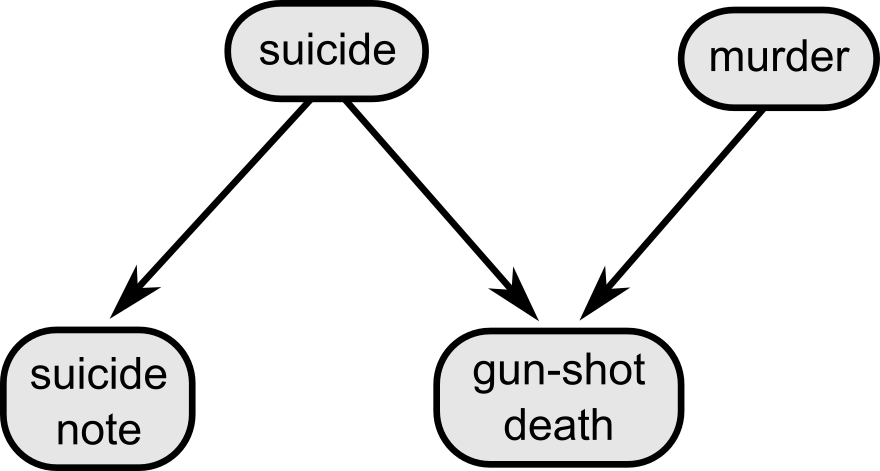
\includegraphics[scale=0.6]{suicide-note-en.png}}}
\end{equation}

At the sub-propositional level, every proposition may be represented as an entity-relation graph, where each node is a \textbf{concept atom}:
\begin{equation}
\vcenter{\hbox{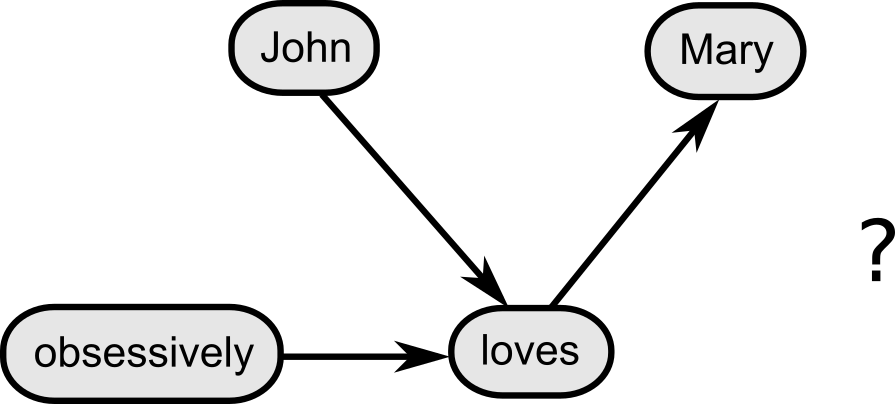
\includegraphics[scale=0.6]{John-loves-Mary-obsessively.png}}}
\end{equation}
but we are still unsure about the exact construction mechanism of sub-propostional graphs.

\subsection{Episodic memory}

Episodic memory = an even-bigger graph?

\section{NN acting on graphs}

\subsection{CNN}

With this analogy:
\begin{equation}
\mbox{CNN for vision} \quad \Longleftrightarrow \quad \mbox{CNN for graphs}
\end{equation}
a new breed of algorithms have been developed, eg: \citep{Niepert2016} \citep{Defferrard2016} \cite{Kipf2016}.  For a nice introduction see the blog entry: \url{https://tkipf.github.io/graph-convolutional-networks/}.

As explained in \citep{Niepert2016}, a CNN works as if a ``receptive field'' moves over an image:
\begin{equation}
\vcenter{\hbox{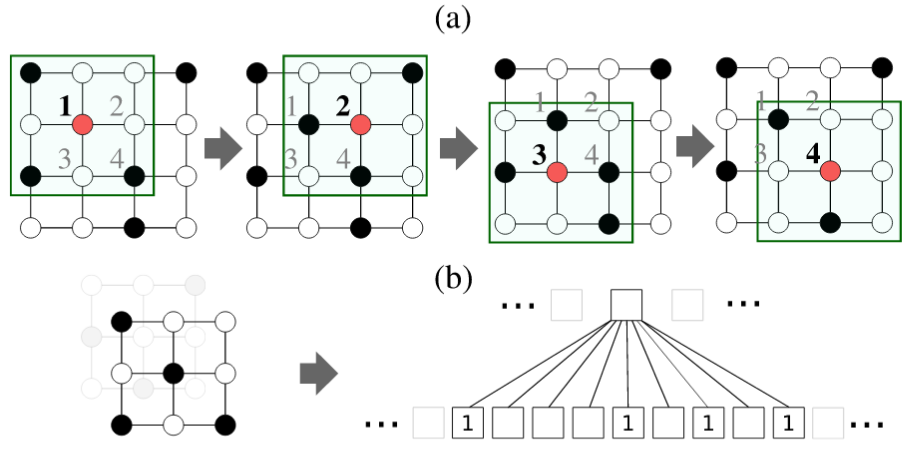
\includegraphics[scale=0.4]{CNN-explained.png}}}
\end{equation}
and the idea is to let a similar receptive field \uline{traverse a graph}.

\section{Cartesian closure}

\ifdefined\chinchin
举例来说,「吃了污糟的食物会肚痛」是一个句子,它经由 $\Eye$ 进入 mental state $\vect{x}$ ,变成 proposition。 但我们希望这逻辑命题变成 $\KB$ 的一部分。With
\else
For example, ``eating dirty food causes stomach pains'' is an NL sentence, it enters from $\Eye$ into the mental state $\vect{x}$, as a \textbf{proposition}.  But we want $\vect{x}$ to become part of $\KB$.  With
\fi
\begin{equation}
\vect{x}' = \vect{f}(\vect{x})
\end{equation}
where \\
\tab $\vect{f} = \KB = \NN$ \\
\tab $\vect{x} = $ state

An individual logic rule is a \uline{restriction} of $\vect{f}$ to a specific input.

$\vect{f} \equiv \KB$ is the \uline{sum of restrictions}:
\begin{equation}
\KB = \bigcup \vect{f}_i
\end{equation}
Or roughly speaking, $\vect{f}$ is the sum total of objects like $\vect{x}$:
\begin{equation}
\vect{f} = \bigcup \vect{x}_i
\end{equation}

However, the problem is that the structure of $\vect{f}$ (as the neural network $\NN$) is too complicated to be expressed as a sum of restricted functions.  This remains an unsolved problem.

\section*{Acknowledgements}

Thanks to Jonathan Yan for suggesting to use CNN for graphs and showed me the relevant papers.

\bibliographystyle{unsrtnat} % or number or aaai ...
\bibliography{AGI-book}

\end{document}
